\chapter{Il progetto stage}
\begin{flushright}
	\parbox{13cm}{\small In questo capitolo vengono presentati i due progetti-clienti su cui si è incentrato lo stage.}
\end{flushright}

\section{Primo progetto}
Il primo progetto graficamente rispecchia molto la versione standard del B2B, ma di fatto include varie funzionalità realizzate appositamente per il cliente.
Innanzitutto, essendo questo portale destinato ad agenti e clienti selezionati, per poterlo utilizzare è necessario essere iscritti. L'iscrizione può avvenire in 2 modalità:
\begin{itemize}
	\item l'amministratore crea un account per l'utente, il quale al primo accesso dovrà cambiare password;
	\item l'utente effettua una richiesta di registrazione, che l'amministratore dovrà approvare per rendere attivo l'account. Questa seconda modalità è attivabile tramite il pannello di configurazione dello stesso amministratore.
\end{itemize}
Una volta in possesso delle credenziali, è quindi possibile accedere al portale. La schermata di login (\hyperref[fig:login1]{figura \ref{fig:login1}}) è la prima pagina a cui si viene indirizzati accedendo al sito tramite URL, sia al primo accesso, sia in caso di sessione già avviata.
\begin{figure}
	\centering
	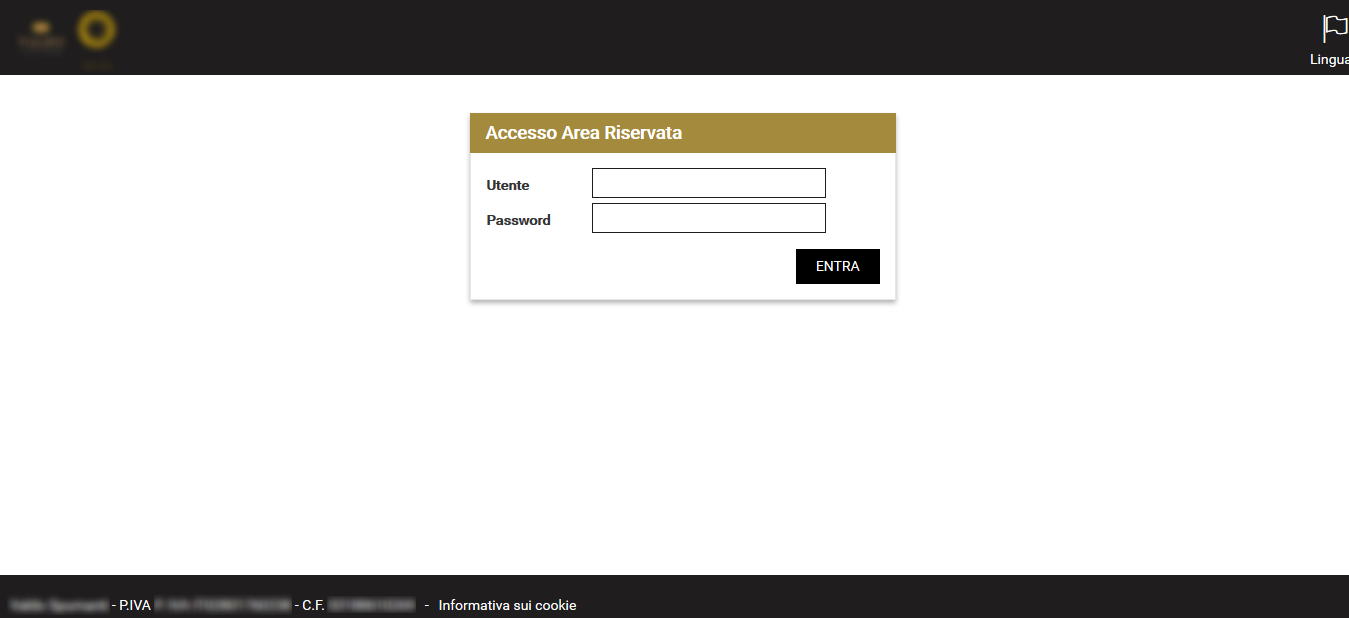
\includegraphics[width=\linewidth]{Immagini/p1/index.png}
	\caption{Pagina di accesso al portale}
	\label{fig:login1}
\end{figure}

Una nota va posta sull'utilizzo delle sessioni. La maggioranza degli oggetti caricati dalla libreria Spring Core sono configurati per essere \textit{session scope}. Questo fa sì che le istanze siano legate agli utenti che utilizzano il B2B, in modo tale da evitare possibili conflitti su nuovi ordini o clienti. Una conseguenza diretta è che non è possibile aprire due finestre dello stesso browser per accedere con utenti diversi. La sessione è inoltre impostata per scadere dopo un certo tempo di inattività, costringendo l'utente a rieffettuare il login, sia per motivi di sicurezza, sia per garantire un maggior controllo sui contenuti, impedendo di concludere operazioni su dati che potrebbero essere deprecati.

Nel corso delle settimane di stage, sono state fatte alcune implementazioni sulla base di richieste del cliente. Generalmente i lavori svolti per questo progetto erano basati su analisi effettuate precedentemente al mio arrivo, in quanto parti dei preventivi presentati al cliente. Prima di iniziare a modificare il codice, mi è tuttavia stato chiesto di presentare in forma di analisi il flusso delle operazioni necessarie per raggiungere l'obiettivo. Le richieste per questo progetto erano legate principalmente all'aggiunta o modifica di informazioni nei risultati o nei parametri di ricerca delle interrogazioni.

Vengono ora presentate alcune delle modifiche effettuate.

\subsection{Codice cliente}
Il codice cliente è un'informazione chiave nel B2B, in quanto contribuisce a costruire ed individuare gli ordini. Dal codice cliente dipendono il tipo dell'ordine, i listini, gli sconti e le promozioni. Per questo motivo poter effettuare ricerche tramite questo codice agevola gli agenti e l'amministrazione. Una delle prime richieste è stata proprio di introdurre questa informazione nei parametri e nei risultati delle interrogazioni.
\begin{figure}
	\centering
	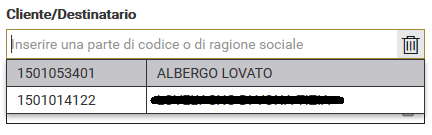
\includegraphics{Immagini/p1/clienti-params.png}
	\caption{Parametri per la ricerca dei clienti}
	\label{fig:clienti-params}
\end{figure}

Per agevolare l'utente nell'inserimento di informazioni corrette, è stato predisposto un campo di testo \virgolette{autocompletante}. Una volta digitati tre caratteri nel campo di input viene eseguita una \textit{query} di ricerca nel database per estrarre la lista dei clienti con codice o descrizione (la ragione sociale nella terminologia del gestionale) contenenti la stringa cercata. Questa \textit{query} deve essere il più ottimizzata possibile, in quanto l'utente non deve subire un rallentamento per un'azione come la ricerca, che ha come scopo quello di far raggiungere più rapidamente gli obiettivi. Un approccio alternativo poteva essere quello di caricare la lista di tutti gli utenti nel \textit{backing bean}, per poi utilizzare i metodi offerti dall'interfaccia \texttt{List} per ottenere la sottolista ricercata.

\subsection{Risultati di ricerca}
Una delle funzionalità più variabili nel B2B è l'ordinamento dei risultati di ricerca, soprattutto nella presentazione dei clienti. Oltre alle modalità di ordinamento comuni (ordine alfabetico o per codice) già predisposti da alcuni componenti Primefaces, che lavora sulle colonne, a volte sono richiesti ordinamenti più complessi.

Nella creazione dell'ordine, la scelta del cliente è solitamente il primo step. I clienti presenti nell'anagrafica sono di due tipi: clienti normali o destinatari. Questi possono poi assumere nella costruzione dell'ordine tre ruoli: cliente di fatturazione, cliente destinatario e, se entrambi i precedenti sono definiti e distinti, è possibile impostare una diversa destinazione. Nello specifico di questo progetto, l'ordinamento richiesto era il seguente: il clienti dovevano essere ordinati alfabeticamente, ma ad ognuno dovevano seguire, se presenti, le varie destinazioni. La lista di partenza era una collezione di \texttt{BusinessPartner}, recuperata direttamente dal database, indistintamente dal ruolo. Per ottenere il risultato voluto sono stati quindi utilizzati i comparatori Java, che permettono di definire per uno stesso oggetto varie regole di ordinamento, utilizzabili poi nelle funzioni di \textit{sorting} offerte dalle collezioni. 
Il risultato è presentato in \hyperref[fig:listaclienti]{figura \ref{fig:listaclienti}}.
\begin{figure}
	\centering
	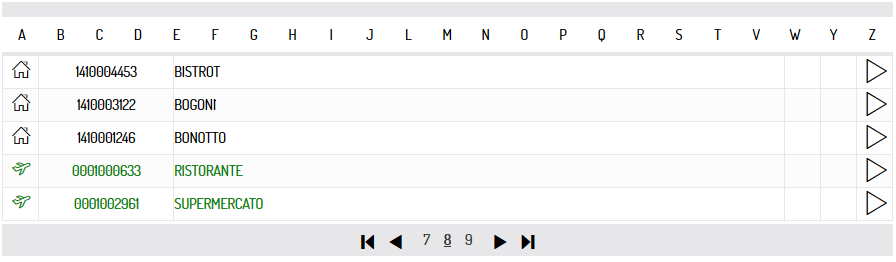
\includegraphics[width=\linewidth]{Immagini/p1/lista-clienti.png}
	\caption{Scelta del cliente nella creazione dell'ordine}
	\label{fig:listaclienti}
\end{figure}

Per rendere più utilizzabile e più accessibile i risultati proposti, questi sono paginati. Primefaces permette di definire il numero di risultati da presentare a priori, indipendentemente dal dispositivo, o dinamicamente, adattando il numero alle dimensioni dello schermo. Questo comportamento dinamico può risultare un vantaggio, in quanto permette di visualizzare il B2B come schermata unica, evitando eventuali scroll che possono nascondere informazioni importanti all'utente, ma anche uno svantaggio, in quanto con dispositivi piccoli e centinaia di risultati possono essere create migliaia di pagine con poche righe; un risultato non proprio efficiente. Per questo motivo per dispositivi come i tablet viene solitamente prefissato il numero di risultati da mostrare.

\subsection{Agenda}
In portali come il B2B, dove sono presenti molte funzionalità, tutte collegate tra loro, il numero di passaggi per completare determinate azioni è importante: per facilitare l'utente nel passaggio tra funzioni diverse è possibile inserire collegamenti tra essi, che riassumano una serie di click altrimenti a carico dell'utente. Uno di questi casi è la creazione di appuntamenti.

In questo progetto è stata richiesta la possibilità di crearli direttamente dalla scheda del cliente, impostando già alcuni parametri per l'evento. Sono stati quindi inseriti dei pulsanti al cui click l'utente viene portato all'agenda e viene creato un appuntamento per il cliente specifico, con la possibilità di inserire direttamente le informazioni mancanti. Una volta inserite queste, l'utente (solitamente l'agente), può salvare l'evento e tornare alla scheda del cliente, o continuare la navigazione. Con un semplice pulsante sono stati riprodotte quindi tre azioni: l'utente clicca sulla voce di menu per aprire l'agenda; l'utente clicca sul pulsante per creare un nuovo evento; l'utente seleziona il cliente desiderato dal campo di input \textit{autocomplete}. Sebbene questa possa essere una caratteristica molto semplice, il B2B è pieno di questi tipi di collegamenti, che permettono di completare attività risparmiando complessivamente molto tempo.

\section{Secondo progetto}
Il secondo progetto su cui si è incentrato lo stage fa parte della categoria dei B2B a sè stanti. Questo progetto è completamente personalizzato e ha ben poco a che fare con lo standard in produzione. Anche se le funzionalità principali sono le stesse, il modo in cui vengono presentate all'utente sono totalmente diverse. Anche graficamente, questo portale rispecchia più gli \textit{e-commerce} B2C piuttosto che gli altri B2B. Essendo così tanto personalizzato, in questo progetto emergono le problematiche analizzate in \hyperref[sec:b2b-smi]{sezione \ref{sec:b2b-smi}}, sia riguardo alla struttura, sia relativamente allo strumento di versionamento correntemente utilizzato.

\subsection{Progettazione}
Per un approccio iniziale con questo progetto il più consapevole possibile sono stati realizzati dei diagrammi delle classi personalizzate per il cliente. La \hyperref[fig:arch-p2]{figura \ref{fig:arch-p2}} rappresenta l'architettura ad alto livello tramite un diagramma dei \textit{package}.
\begin{figure}[H]
	\centering
	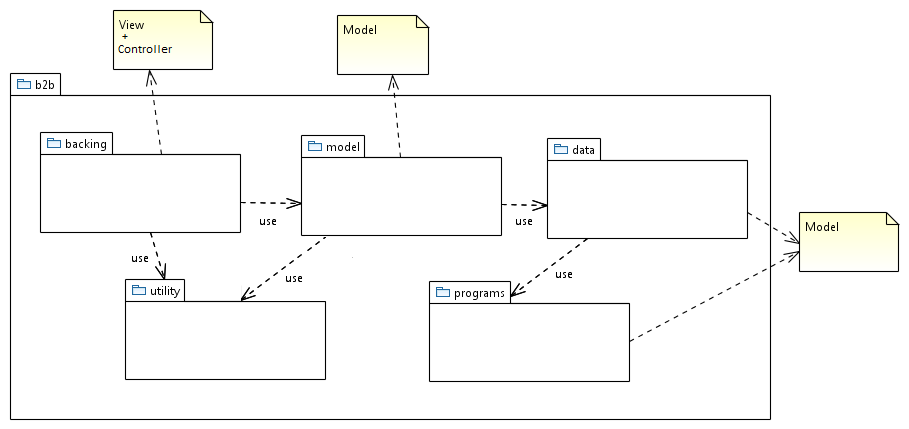
\includegraphics[width=\linewidth]{Immagini/p2/architettura.png}
	\caption{Architettura generale del secondo progetto}
	\label{fig:arch-p2}
\end{figure}

Vengono ora riportati i diagrammi delle classi per i \textit{package} dei \textit{backing bean} (\hyperref[fig:bck]{figura \ref{fig:bck}}), dei \textit{manager} (\hyperref[fig:manager]{figura \ref{fig:manager}}) e dei \textit{data provider} (\hyperref[fig:data]{figura \ref{fig:data}}). Nei diagrammi, che riportano solo le classi personalizzate, si può vedere come ogni tipo di entità abbia i corrispettivi oggetti nei vari \textit{package}. Non sono riportate le relazioni tra le classi in quanto richiederebbero un diagramma troppo grande per presentarlo in questa relazione; i seguenti hanno quindi lo scopo di mostrare applicati i concetti presentati in \hyperref[sec:b2b-struttura]{sezione \ref{sec:b2b-struttura}}.
\begin{figure}[H]
	\centering
	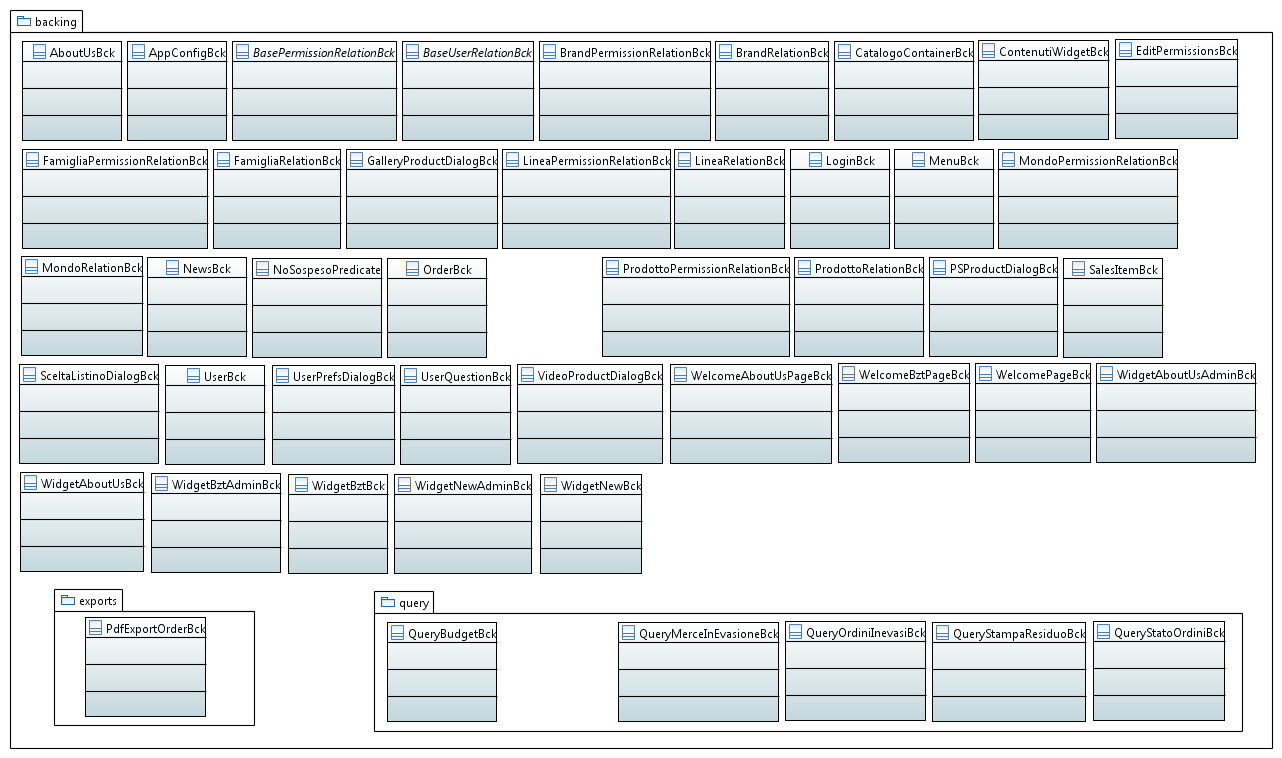
\includegraphics[height=\linewidth,angle=90]{Immagini/p2/bck.png}
	\caption{\textit{Backing bean} personalizzati}
	\label{fig:bck}
\end{figure}
\begin{figure}[H]
	\centering
	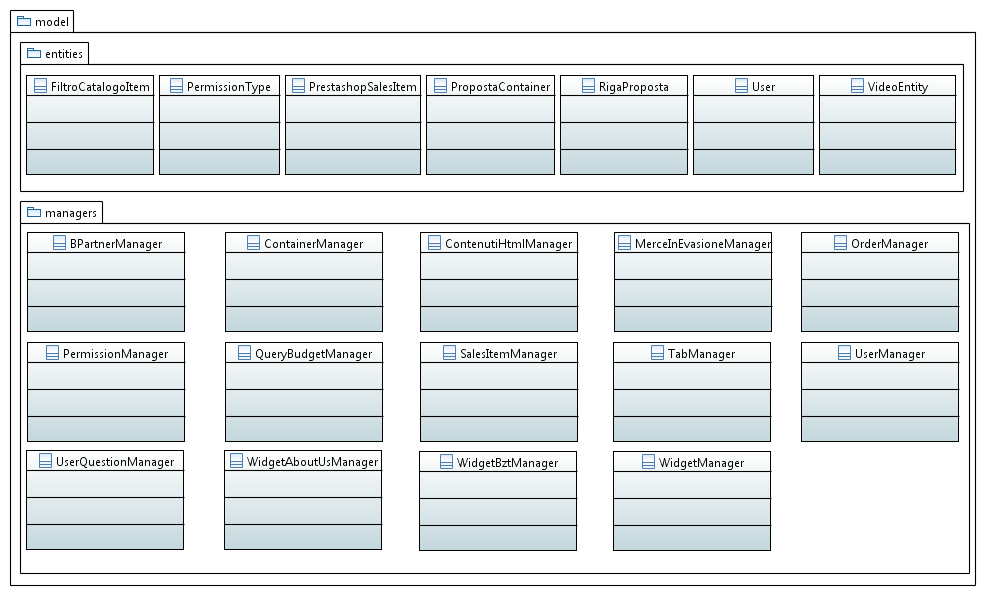
\includegraphics[height=0.9\linewidth,angle=90]{Immagini/p2/manager.png}
	\caption{\textit{Manager} e entità personalizzati}
	\label{fig:manager}
\end{figure}
\begin{figure}[H]
	\centering
	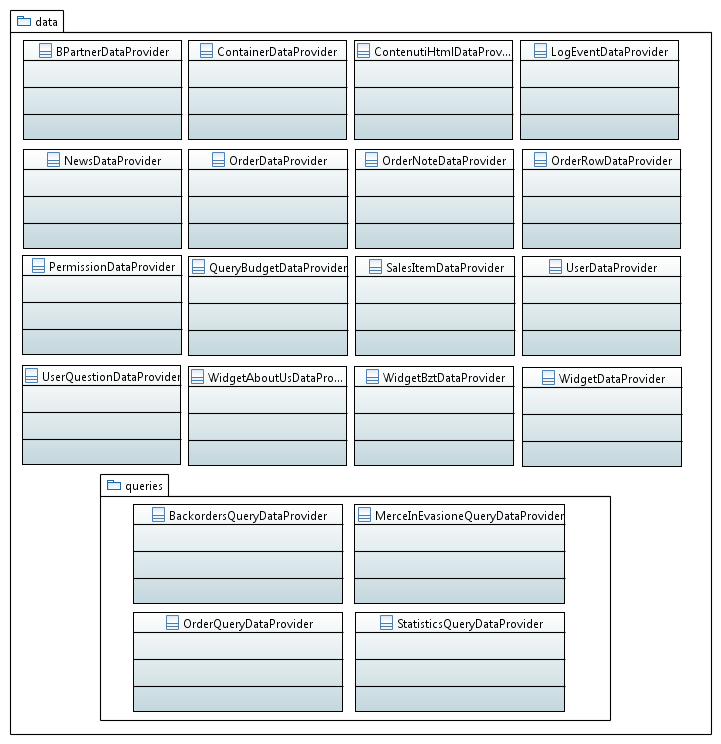
\includegraphics[width=\linewidth]{Immagini/p2/data.png}
	\caption{\textit{Data provider} personalizzati}
	\label{fig:data}
\end{figure}


\subsection{Task per invio di newsletter}
Una delle funzionalità create per questo progetto è un task per l'invio di newsletter riguardo a nuove offerte disponibili sul portale. Per realizzare questo compito è stata estesa la classe \texttt{ExtendedTask} del pacchetto standard, che si occupa di creare un thread il cui avvio è programmabile tramite interfaccia grafica. Il task si occupa di recuperare dal database le nuove proposte disponibili per tipologia, quindi carica l'elenco dei destinatari, a seconda della lingua carica e traduce il template del messaggio, lo compila con i dati corretti e infine lo invia al gruppo di destinatari il cui locale (inteso come il gruppo di parametri che definisce la lingua, il paese e qualsiasi altra variante specifica, scelti dall'utente per la visualizzazione dell'interfaccia) corrisponde alla lingua di traduzione del template.

Il recupero delle informazioni avviene anch'esso seguendo alcuni passaggi:
\begin{itemize}
	\item vengono caricate dal database tutte le proposte con data di inizio validità corrispondente al parametro di configurazione del task, settabile tramite interfaccia grafica e di default corrispondente al giorno successivo alla data di sistema;
	\item delle proposte risultanti vengono quindi caricate le immagini dei prodotti;
	\item l'elenco dei prodotti viene ordinato per tipologia.
\end{itemize}
Poiché il numero di proposte è molto variabile, il template è costruito con un unico prodotto per categoria. Questo viene poi replicato tante volte quante sono le proposte o eliminato nel caso in cui non ve ne siano. In questo caso viene eliminata anche la sezione relativa.


\subsection{Export log utenti}
Sapere cosa fanno gli utenti e quali sono le funzionalità più utilizzate sono un aspetto importante per chi gestisce il B2B, in quanto permette di favorirne l'utilizzo e quindi la soddisfazione degli utenti stessi. Inoltre, sapere quali utenti utilizzano maggiormente il portale fa sì che possano essere applicate promozioni o condizioni di vendita a loro mirate. L'utilizzo di log per gli eventi che riguardano gli utenti è quindi un vantaggio notevole per l'amministrazione, che grazie ad essi ha un nuovo modo di conoscere i propri agenti e clienti, oltre che tramite gli ordini effettuati.

L'analisi di questo tipo di dati è effettuata tramite l'esportazione dei log sotto forma di fogli di calcolo. Anche in questo caso sono disponibili vari parametri di ricerca per risultati più precisi, come ad esempio il tipo di evento, il nome utente, le date di inizio e fine periodo. Viene anche data la possibilità di effettuare vari tipi di esportazione, a seconda del numero di dati che si vogliono avere: il riepilogo permette di tener traccia della quantità di operazioni effettuate dagli utenti, indipendentemente dalla tipologia; l'export normale comprende i tipi di operazioni e informazioni specifiche sul tipo di operazione, come ad esempio lo \textit{user agent} del browser utilizzato che, nonostante non costituisca un'informazione precisa ed assoluta, è comunque indicativa; l'export completo, infine, comprende un numero molto maggiore di informazioni, soprattutto rispetto a dati specifici degli utenti.

\subsection{Ottimizzazione query}
Allo sviluppo di questa funzionalità è seguito un lavoro di ottimizzazione delle \textit{query} presenti per il recupero dei dati dal database. In particolare, nell'esportazione dei prodotti viene creato un file contenente migliaia di elementi. La modalità con cui venivano reperiti i prodotti rendeva il processo di creazione estremamente lungo, richiedendo parecchi minuti di caricamento. L'obiettivo era quindi quello di ridurre questo tempo di esecuzione, ottimizzando sia le \textit{query} che il caricamento delle immagini. 

Il risultato è stato ottenuto limitando gli accessi alle due fonti dei dati, sfruttando i \textit{prepared statement} per creare interrogazioni che, nonostante la maggior complessità rispetto alle precedenti, con tempi di esecuzione relativi anche più lunghi, risultavano complessivamente più precise e più rapide. Allo stesso modo il caricamento delle immagini è stato reso massivo e non più a livello individuale per prodotto. Come risultato finale è stato raggiunto un dimezzamento dei tempi per la creazione del primo \textit{export}, mentre le successive richieste sono ora eseguite in pochi secondi.

\section{I due progetti a confronto}
I due progetti sono dunque molto diversi tra loro, nonostante la base sia la stessa. La prima e più evidente differenza è la grafica e ciò dipende oltre che dal tipo di prodotti anche dalla professione del personale addetto alla gestione del B2B. Mentre per il primo progetto ad occuparsi del portale è un responsabile \Gls{CED}, per il secondo progetto il referente è un grafico. Questo ha determinato un'attenzione molto maggiore ai dettagli grafici, a volte anche a scapito dell'usabilità. Vengono ora presentate alcune delle funzionalità comuni, evidenziandone le differenze.

\subsection{Ricerca interrogazioni}
Il pannello di ricerca delle interrogazioni è probabilmente l'unica cosa che i due progetti hanno in comune (\hyperref[fig:params-1]{figura \ref{fig:params-1}} e \hyperref[fig:clienti-params-2]{figura \ref{fig:clienti-params-2}}). Nel secondo progetto però vi è una divergenza nel modo in cui il componente è presentato all'interno delle varie interrogazioni. Per alcune è stato deciso di inserire le \textit{label} dopo ai campi di input (\hyperref[fig:params-2]{figura \ref{fig:params-2}}). Questo tipo di presentazione può creare confusione anche per un utilizzatore consuetudinario, che nelle altre interrogazioni, negli altri \textit{e-commerce} e in generale in qualsiasi altro sito web, è abituato a vedere le etichette descrittive sopra o a sinistra dei relativi campi.
\begin{figure}[H]
	\centering
	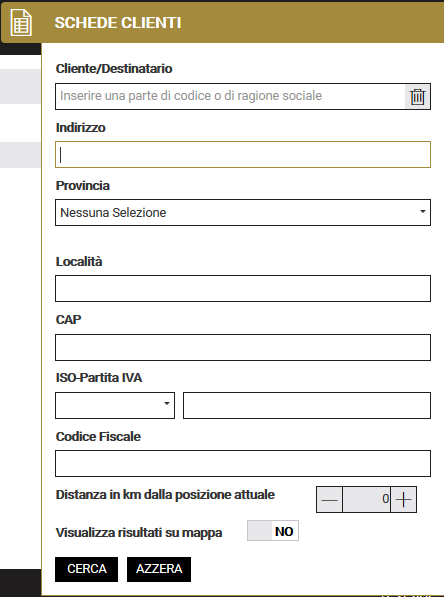
\includegraphics[height=0.8\linewidth]{Immagini/p1/params.png}
	\caption{Form di ricerca per il progetto 1}
	\label{fig:params-1}
\end{figure}
\begin{figure}[H]
	\centering
	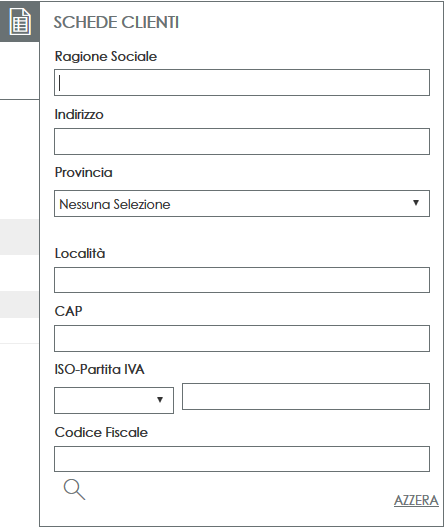
\includegraphics[height=0.7\linewidth]{Immagini/p2/clienti-params.png}
	\caption{Form di ricerca clienti per il progetto 2}
	\label{fig:clienti-params-2}
\end{figure}
\begin{figure}[H]
	\centering
	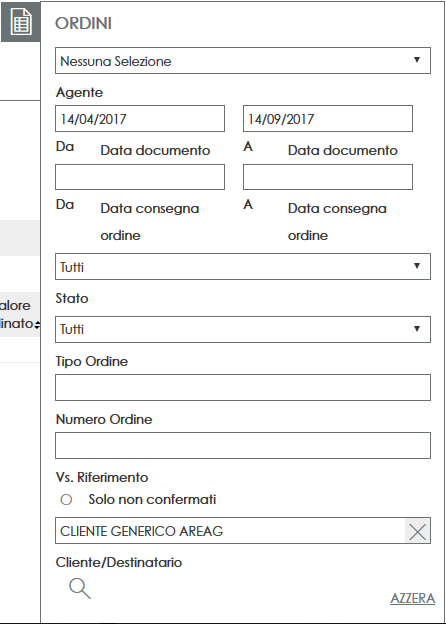
\includegraphics[height=0.8\linewidth]{Immagini/p2/params.png}
	\caption{Form di ricerca ordini per il progetto 2}
	\label{fig:params-2}
\end{figure}

\subsection{Catalogo prodotti}
Anche la presentazione dei prodotti a catalogo è nettamente differente. Per il primo progetto i prodotti sono presentati in un elenco (\hyperref[fig:catalogo-1]{figura \ref{fig:catalogo-1}}), raggruppati per categoria. Nel secondo progetto invece è stato scelto un catalogo molto più simile a quello degli \textit{e-commerce} B2C. In entrambi i progetti i prodotti sono visualizzabili anche senza aver creato un ordine. Nel secondo progetto essi sono raggruppati per categorie generiche, come \virgolette{novità} o \virgolette{outlet}e nel tipo di presentazione a griglia (\hyperref[fig:catalogo-2]{figura \ref{fig:catalogo-2}}) grande importanza è data all'immagine del prodotto, che risulta fondamentale nell'ambito di vendita del cliente, l'arredamento.
\begin{figure}[H]
	\centering
	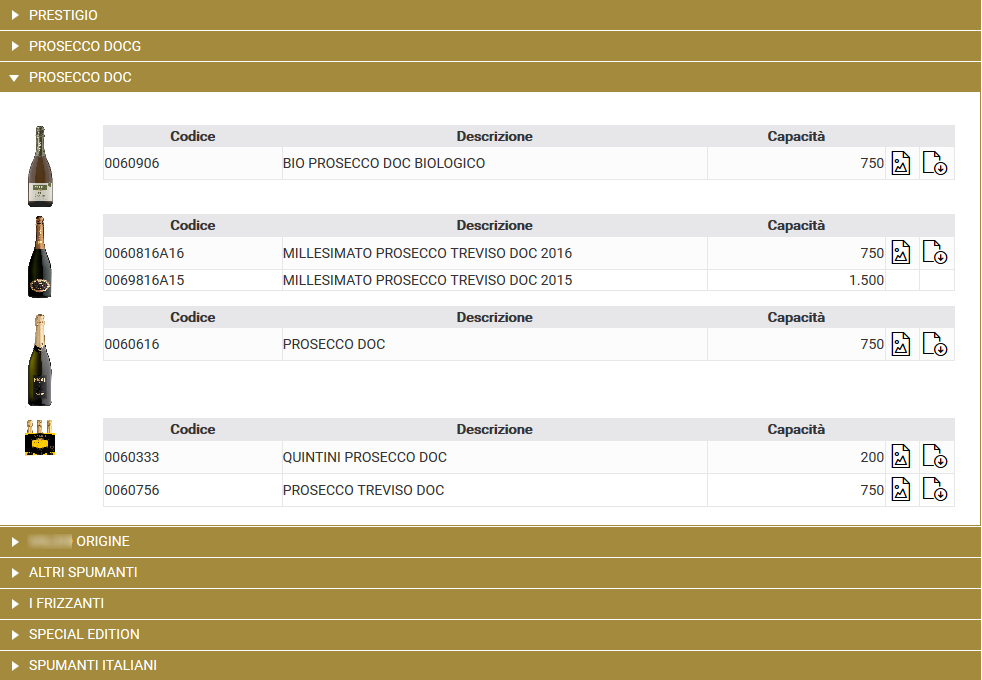
\includegraphics[width=\linewidth]{Immagini/p1/catalogo.png}
	\caption{Presentazione dei prodotti nel progetto 1}
	\label{fig:catalogo-1}
\end{figure}
\begin{figure}[H]
	\centering
	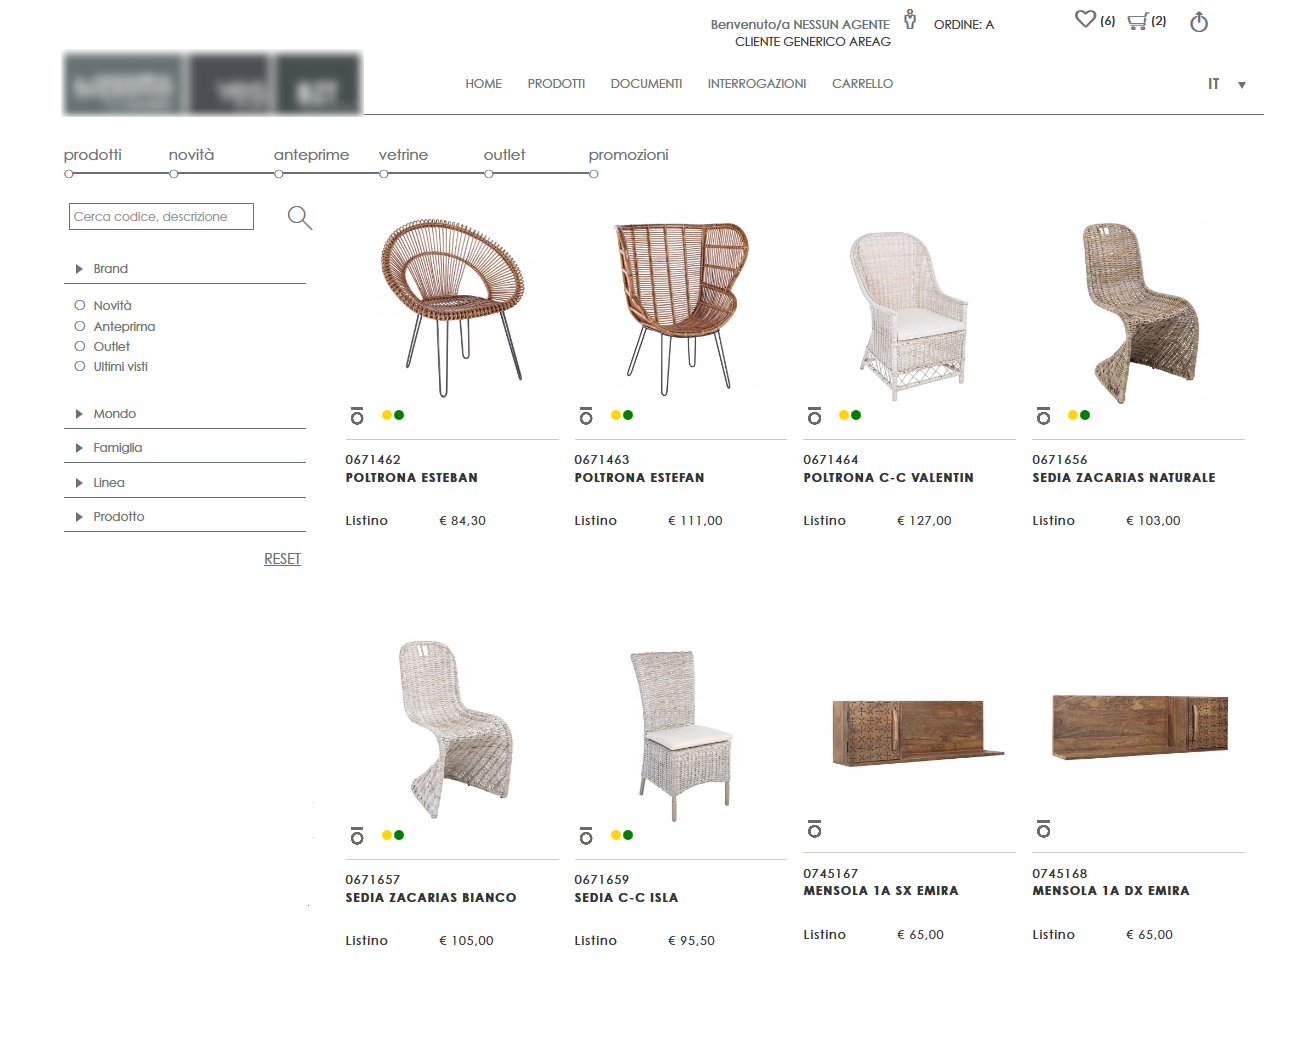
\includegraphics[width=\linewidth]{Immagini/p2/catalogo.png}
	\caption{Presentazione dei prodotti nel progetto 2}
	\label{fig:catalogo-2}
\end{figure}

\subsection{Creazione dell'ordine}
Anche il processo di creazione dell'ordine è differente per le due versioni del B2B. Nel primo progetto viene riproposto il procedimento standard, attraverso un \textit{wizard} che permette di comporre l'ordine. Ai passi standard sono aggiunti quelli personalizzati, ad esempio per l'inserimento di premi o promozioni. Nel secondo caso, invece, l'ordine prima di essere inviato è definito \virgolette{carrello}. È quindi possibile creare e gestire più carrelli contemporaneamente. Per entrambi i progetti l'ultimo step prima di confermare l'ordine e inviarlo al gestionale è il riassunto dell'ordine, un comportamento in comune anche con altri siti web e che permette all'utente di controllare le informazioni un'ultima volta. Da questa schermata è possibile anche rifinire gli ultimi dettagli.

Nonostante la funzione in comune, anche in questo caso la presentazione è totalmente differente. Nel primo progetto è stata richiesta la possibilità di inserire tutte le informazioni riguardanti il cliente di fatturazione e di spedizione prima di inviare l'ordine, tra cui il pagamento e i contatti. I dati dovevano inoltre essere compressi per rientrare in una schermata singola (sia per utilizzo tramite computer che, per quanto possibile, da tablet). Il risultato è presentato in \hyperref[fig:summary-1]{figura \ref{fig:summary-1}}.
\begin{figure}[H]
	\centering
	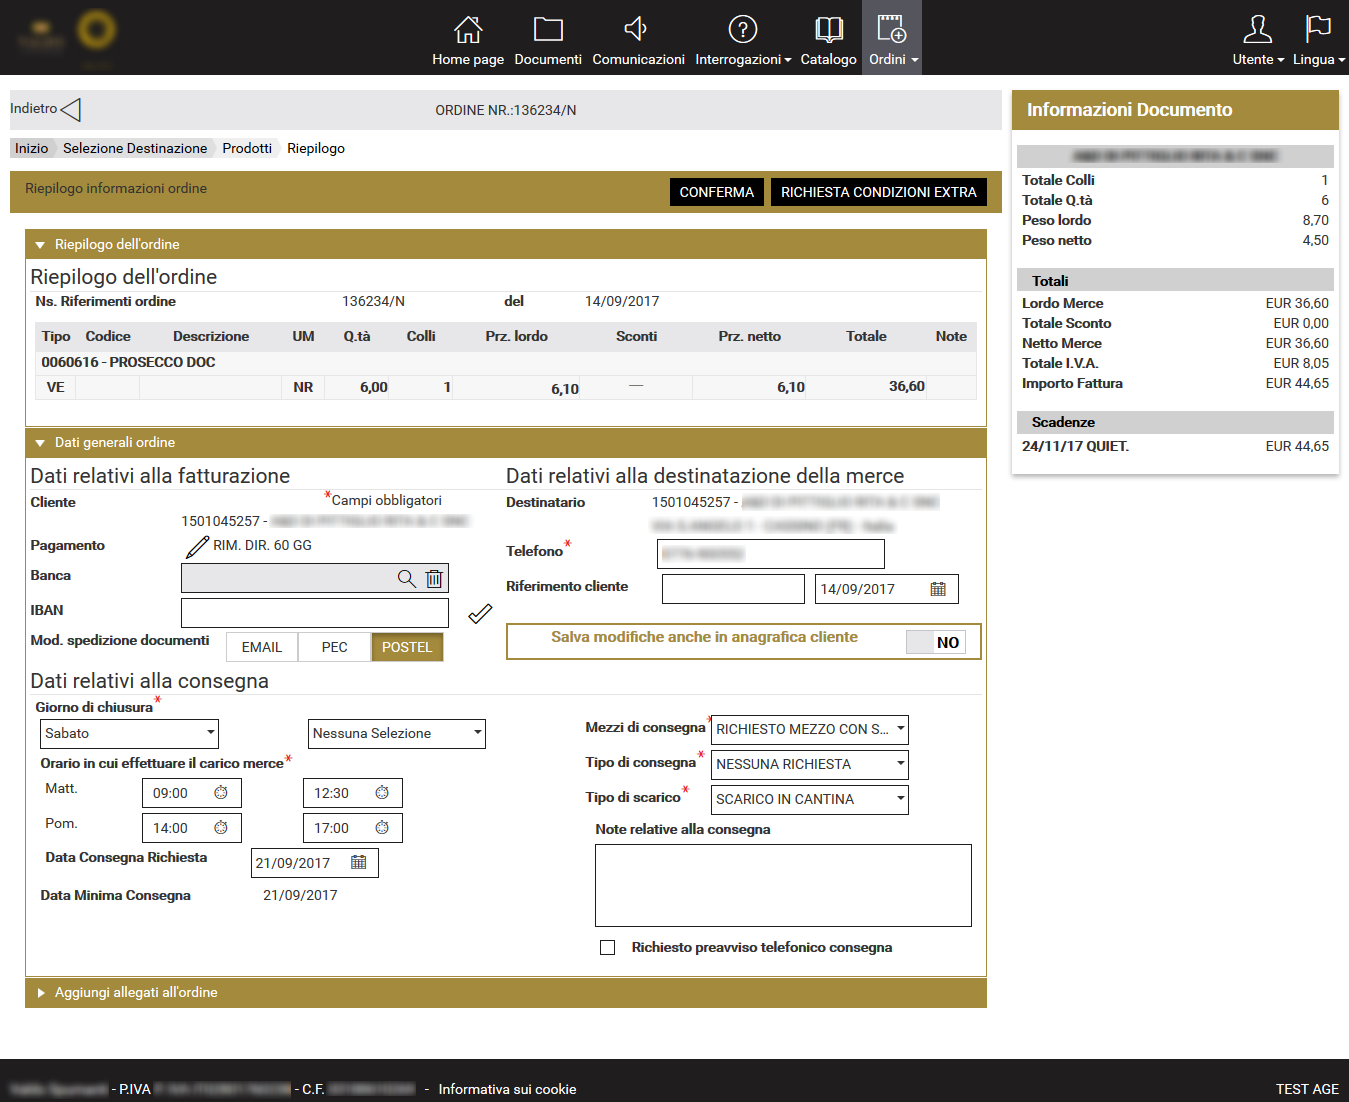
\includegraphics[width=\linewidth]{Immagini/p1/summary.png}
	\caption{Schermata riepilogativa del progetto 1}
	\label{fig:summary-1}
\end{figure}
Nel secondo progetto invece, il riepilogo dell'ordine è del tutto statico (\hyperref[fig:summary-2]{figura \ref{fig:summary-2}}). Tutte le eventuali modifiche vanno quindi effettuate tornando al carrello.
\begin{figure}[H]
	\centering
	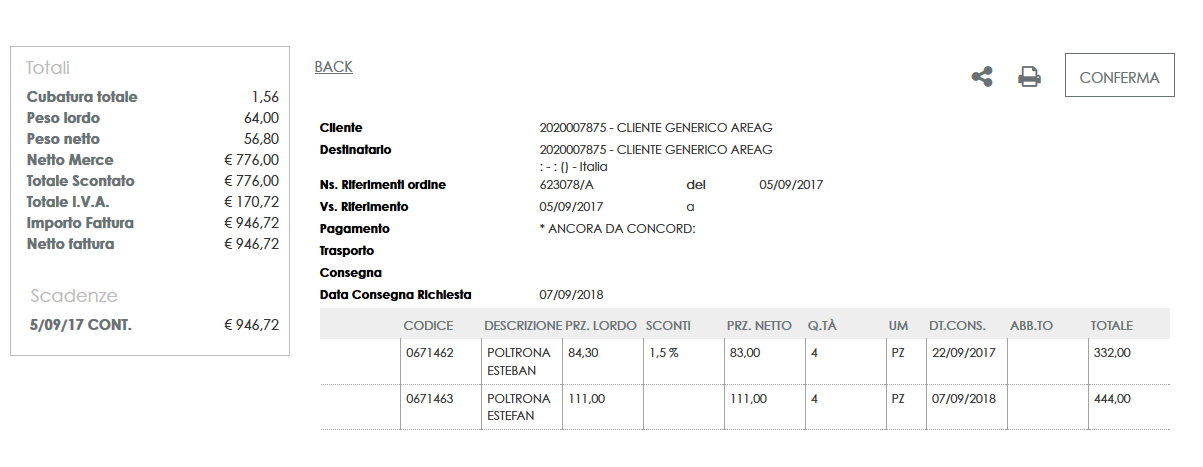
\includegraphics[width=\linewidth]{Immagini/p2/summary.png}
	\caption{Schermata riepilogativa del progetto 2}
	\label{fig:summary-2}
\end{figure}

Una nota va posta sulla pagina che permette di modificare i carrelli (\hyperref[fig:carrello-2]{figura \ref{fig:carrello-2}}), ed in particolare sulla visualizzazione dei dati di testata. I dati sono contenuti in un form, modificabile dall'utente. Il problema è che il cliente ha voluto rimuovere tutti i segnali che tali parametri sono in realtà campi di input, violando di fatto tutte le convenzioni del web. In \hyperref[fig:carrello-form]{figura \ref{fig:carrello-form}} è presentato il modulo, dove i campi editabili sono i valori della data consegna richiesta e delle note.
\begin{figure}[H]
	\centering
	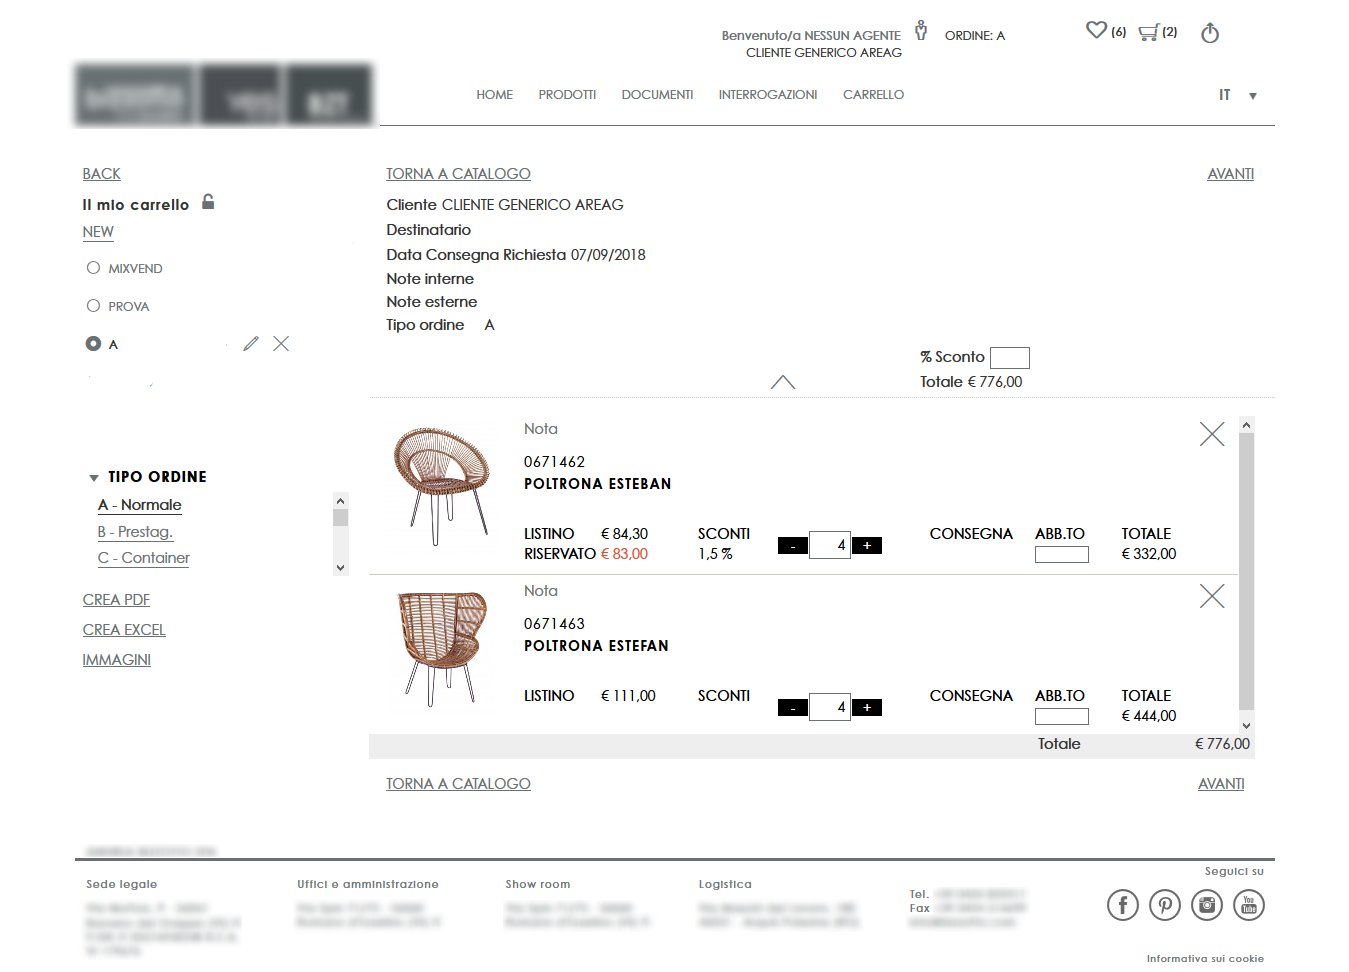
\includegraphics[width=\linewidth]{Immagini/p2/carrello.png}
	\caption{Pagina di gestione del carrello per il progetto 2}
	\label{fig:carrello-2}
\end{figure}
\begin{figure}[H]
	\centering
	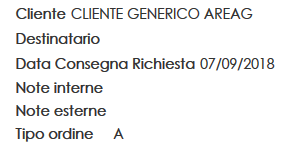
\includegraphics[width=0.5\linewidth]{Immagini/p2/carrello-form.png}
	\caption{Form di modifica dei dati di testata dell'ordine}
	\label{fig:carrello-form}
\end{figure}